\section{Methodology}

%\begin{enumerate}
%	\item 4 shots of grid: 1. LE 2. TE 3. near-field for entire shape 4. the entire grid domain. Note: should show T-rex feature that was used
%	\item table 1: cell count and normal-to-wall spacing used, list BC, list reference values, list submodels chosen (i.e. viscous model), provide numerical scheme and spacial accuracy
%\end{enumerate}

\subsection{Screenshots of grid}

\begin{figure}[H]
	\centering
	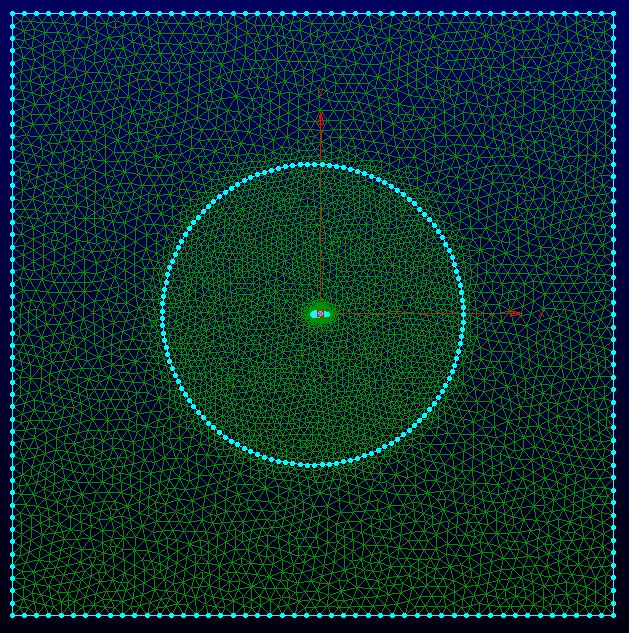
\includegraphics[width=\textwidth]{general_images/farfield}
	\caption{Farfield}
\label{fig:farfield}
\end{figure}

\begin{figure}[H]
	\centering
	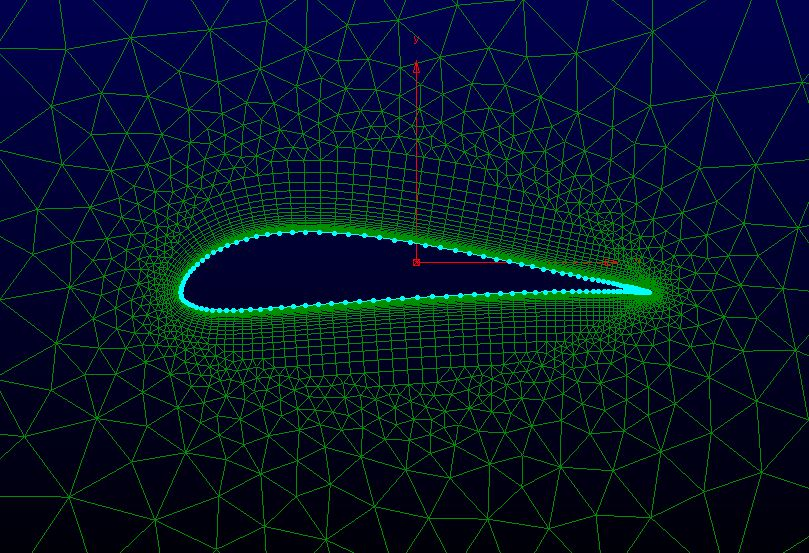
\includegraphics[width=0.9\textwidth]{general_images/nearfield}
	\caption{Nearfield}
\label{fig:nearfield}
\end{figure}	

\begin{figure}[H]
	\centering
	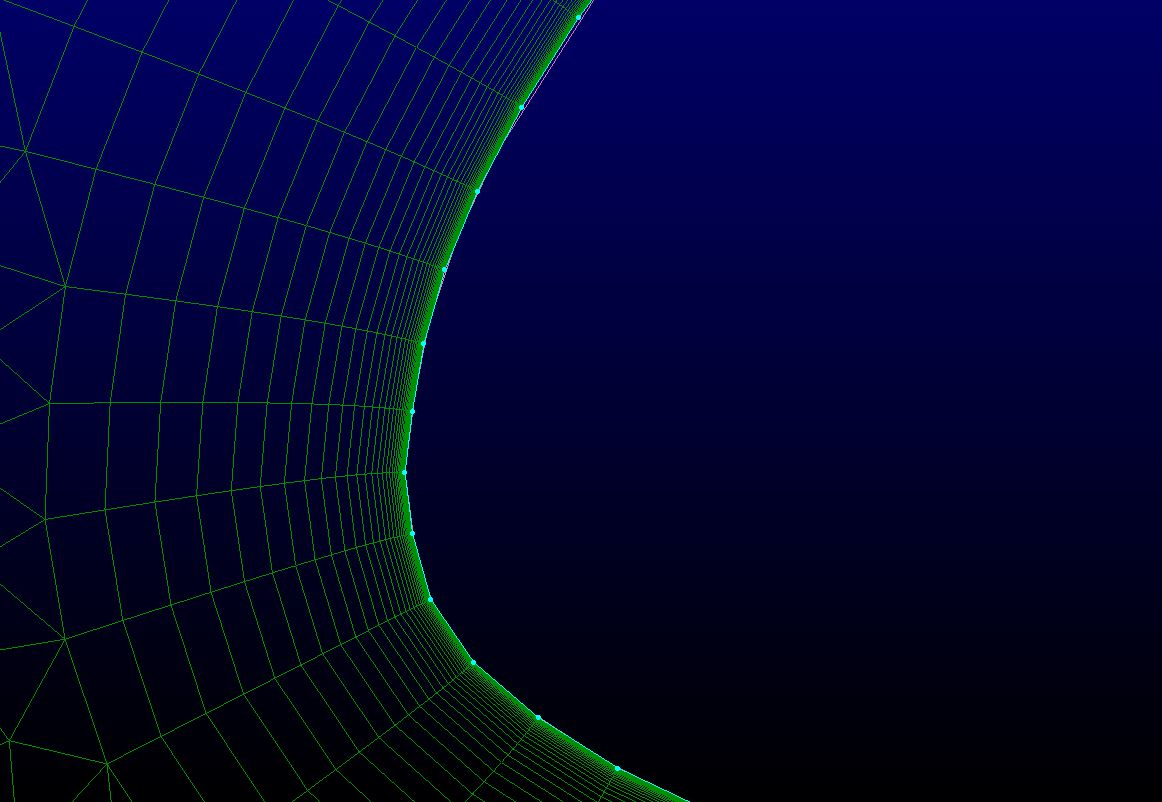
\includegraphics[width=0.9\textwidth]{general_images/LE1}
	\caption{Leading edge zoomed-in view}
\label{fig:LE}
\end{figure}


\begin{figure}[H]
	\centering
	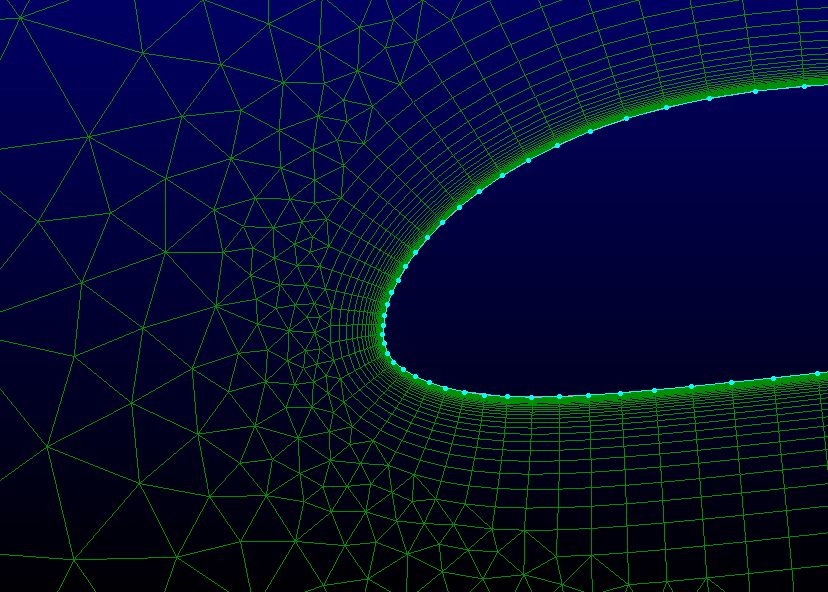
\includegraphics[width=0.9\textwidth]{general_images/LE2}
	\caption{Leading edge zoomed-out view}
\label{fig:LE}
\end{figure}


\begin{figure}[H]
	\centering
	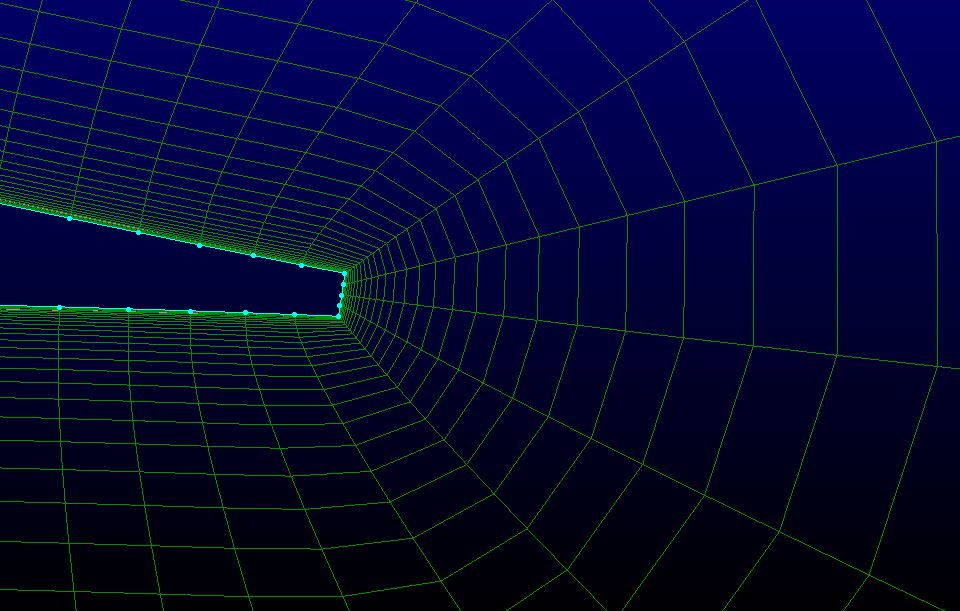
\includegraphics[width=0.9\textwidth]{general_images/TE2}
	\caption{Trailing edge zoomed-in view}
\label{fig:TE}
\end{figure}

\begin{figure}[H]
	\centering
	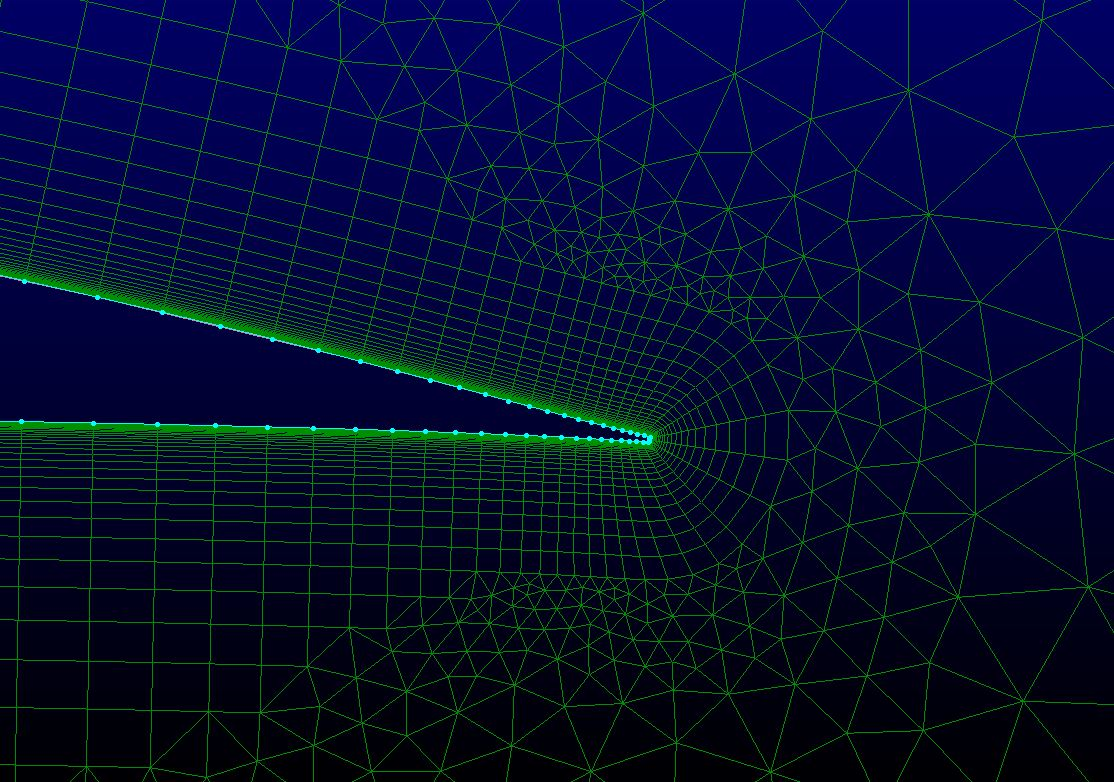
\includegraphics[width=0.9\textwidth]{general_images/TE1}
	\caption{Trailing edge zoomed-out view}
\label{fig:TE}
\end{figure}

\begin{table}[H]
\caption{General grid information}
	\centering
	\begin{tabular}{|l|p{4.5in}|} \hline
%				 & Value \\ \hline \hline
		Cell count & \textbf{Inner mesh} (i.e. rotated grid): 11,890\newline \textbf{Outer mesh} (i.e. stationary grid): 6204 \\ \hline
		Normal-to-wall spacing & $\boldsymbol{\Delta}$\textbf{s} = 1e-5 \\ \hline
		Boundary conditions & \textbf{Left edge}: velocity inlet \newline \textbf{Right edge}: pressure outlet \newline \textbf{Airfoil surface}: wall \newline \textbf{Upper and lower grid edge}: tunnel \\ \hline
		Reference values & \textbf{Area}: 1 [m$^2$] \newline \textbf{Density}: 1.225 [kgm$^{-3}$] \newline \textbf{Pressure}: 101,325 [Pa] \newline \textbf{Temperature}: 298 [K] \newline \textbf{Velocity}: 17.88 [m/s] \newline \textbf{Viscosity}: 1.789e-05 [kgm$^{-1}$s$^{-1}$] \newline \textbf{Ratio of specific heat}: 1.4 \\ \hline
		Submodels & \textbf{Viscous}: transitional SST \\ \hline
		Numerical Schemes & \textbf{Gradient}: least-squares cell based \newline \textbf{Pressure}: second order \newline \textbf{Momentum}: second order upwind \newline \textbf{Turbulent kinetic energy}: first order upwind \newline \textbf{Specific dissipation rate}: first order upwind \newline \textbf{Intermittency}: first order upwind \newline \textbf{Momentum thickness Re}: first order upwind \\ \hline
	\end{tabular}
\end{table}



% gradient: least squares cell based
% pressure: second order
% momentum: second order upwind
% turbulent kinetic energy: first order upwind
% specific dissipation rate: first order upwind
% intermittency: first order upwind
% momentum thickness Re: first order upwind